% Gemini theme
% https://github.com/anishathalye/gemini

\documentclass[final]{beamer}

% ====================
% Packages
% ====================

\usepackage[T1]{fontenc}
\usepackage{lmodern}
%\usepackage[size=custom,width=70,height=112,scale=1.0]{beamerposter} %841 & 1189 mm
\usepackage[orientation=portrait, size=a0, scale=1.3]{beamerposter}
\usetheme{gemini}
\usecolortheme{gemini}
\usepackage{graphicx}
\usepackage{booktabs}
\usepackage{tikz}
\usepackage{pgfplots}

% ====================
% Lengths
% ====================

% If you have N columns, choose \sepwidth and \colwidth such that
% (N+1)*\sepwidth + N*\colwidth = \paperwidth
\newlength{\sepwidth}
\newlength{\colwidth}
\newlength{\twocolwidth}
\setlength{\sepwidth}{3cm}%{0.025\paperwidth}
\setlength{\colwidth}{24cm}%{0.3\paperwidth}
\setlength{\twocolwidth}{51cm}%{0.625\paperwidth}

\newcommand{\separatorcolumn}{\begin{column}{\sepwidth}\end{column}}

% ====================
% Title
% ====================

\title{GRAPE: Handling Missing Data using Graph Representation Learning}

%\author{Rabin Thapa \and Alina Lazar}
\author{Rabin Thapa \and Alina Lazar}
\institute[shortinst]{ Youngstown State University}

% ====================
% Body
% ====================
\pgfplotsset{compat=1.15}
%\beamertemplategridbackground[1cm]
\begin{document}
\addtobeamertemplate{headline}{} 
{\begin{tikzpicture}[remember picture, overlay]
\node [anchor=north east, inner sep=1cm] (ysu)  at (75.1,6.3)
{
\includegraphics[height=5cm,width=10cm]{figures/quest.png}};
\node [anchor=north west, inner sep=1cm] (ysu)  at (10,6.3)
{
\includegraphics[height=5cm,width=9cm]{figures/ysu_logo.jpg}};
	\end{tikzpicture}}


\begin{frame}[t]
\hspace{2cm}
\begin{columns}[t]
\separatorcolumn
\begin{column}{\colwidth}
  \begin{block}{Abstract}
    %\begin{figure}
    %  \centering
    %  \begin{tikzpicture}[scale=6]
    %    \draw[step=0.25cm,color=gray] (-1,-1) grid (1,1);
    %    \draw (1,0) -- (0.2,0.2) -- (0,1) -- (-0.2,0.2) -- (-1,0)
    %      -- (-0.2,-0.2) -- (0,-1) -- (0.2,-0.2) -- cycle;
    %  \end{tikzpicture}
    %  \caption{A figure caption.}
    %\end{figure}

Handling missing data has been an important preprocessing step for many machine learning tasks. However, existing imputation models tend to have strong prior assumptions and cannot learn from downstream tasks. In this project, we evaluate a graph-based framework known as GRAPE for data imputation.

To evaluate the performance of GRAPE framework, we experiment it on several benchmark datasets and show its accuracy in terms of root mean square error (\textit{rmse}) and compare it with existing state-of-the-art methods. 

  \end{block}

  \begin{block}{The GRAPE Framework}
GRAPE formulates a missing value problem using graph representation, where the observations and features are viewed as two types of nodes in a \testbf{bipartite graph}, and the observed feature values as edges between them. The \textit{feature imputation} is formulated as an \textit{edge-level prediction} task and the \textit{label prediction} as a \textit{node-level prediction} task (see Figure 2).

GRAPE solves both tasks via Graph Neural Networks (GNNs). Its core architecture is inspired by the GraphSAGE model from which it inherits inductive learning capabilities across different graphs.


  \end{block}

% could include this in datasets and experiments
  \begin{block}{Datasets and Experiments}
  
The experiments are conducted on seven datasets (naval, power, energy, kin8nm, concrete, energy, and housing) obtained from UCI Machine Learning Repository. The missing values are introduced by removing random values in the data matrix. It is done by using a \textit{mask}, and the proportion of masked values in a dataset is called \textit{missing ratio}.

Figure 1 shows concrete dataset which has 1029 observations and 9 features. The white spaces denote missing values (with \textit{missing ratio} of 0.10).
%write about masking techniques
 \begin{figure}
 	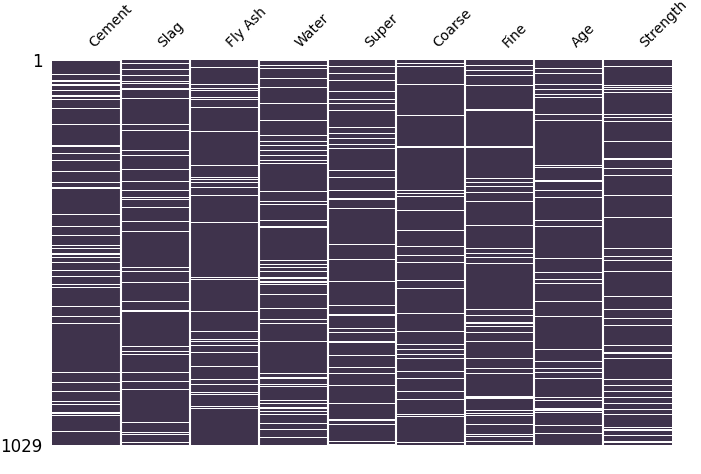
\includegraphics[width=1.04\textwidth]{figures/missing_plot.png}
 	\caption{Concrete dataset showing missing values}
 	\label{cdft}
 \end{figure}
  \end{block}

%write about GRAPE configurations
Furthermore, all the experiments are conducted with following configurations:
\begin{itemize}
    \item 20,000 training epochs using Adam optimizer with a learning rate of 0.001 \item Activation function: RELU
    \item feature imputation tasks: 3-layer GNN with 64-hidden units
    \item label prediction tasks: 2-layer GNN with 16 hidden units
\end{itemize}
\end{column}

\separatorcolumn
\begin{column}{\twocolwidth}
\begin{figure}
	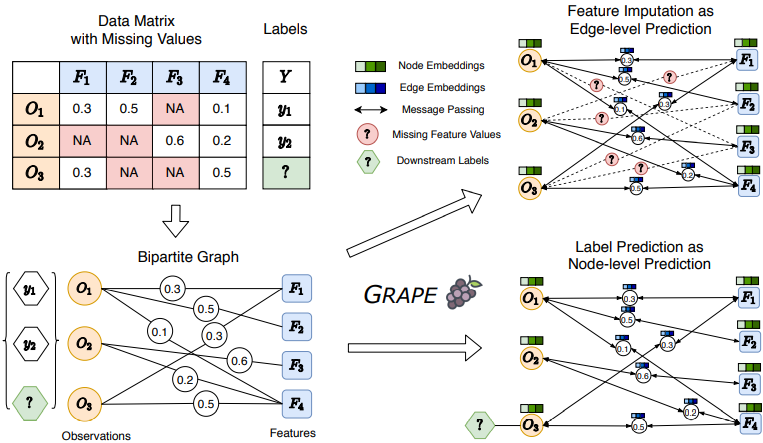
\includegraphics[width=1\textwidth,height=0.5\textwidth]{figures/GRAPE_Framework.png}
	\caption{Overview of the proposed GRAPE framework}
	\label{fig:approach}
\end{figure}


\separatorcolumn
\vspace{-3cm}
\begin{columns}[t, totalwidth=\twocolwidth]
\begin{column}{\colwidth}

  \begin{block}{Model Evaluation}
  \testbf{Feature imputation:} Figure 3 shows how the values of different test metrics change as the number of epochs increases.

     \begin{figure}
 	    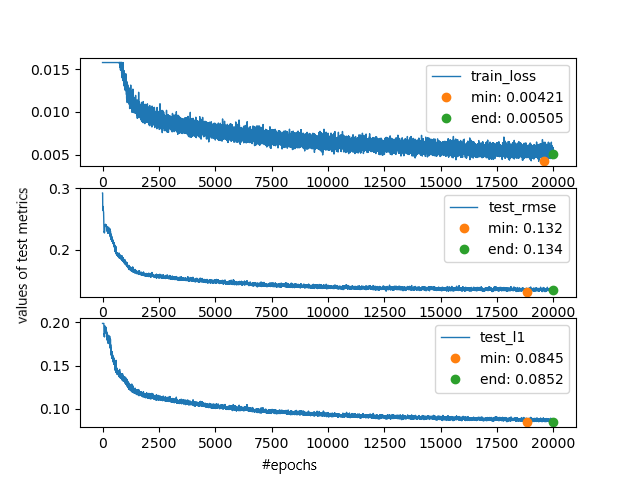
\includegraphics[width=1\textwidth]{figures/curves.png}
 	    \caption{Values of test metrics across different epochs}
 	    \label{cdft}
    \end{figure}
  
  Figure 4 compares \textit{rmse} values of feature imputation for GRAPE against other commonly known imputation methods. The test metric is chosen to be the root mean square error (\textit{rmse}) between predicted and actual values (wherever the actual values are masked for testing).
  
   \begin{figure}
 	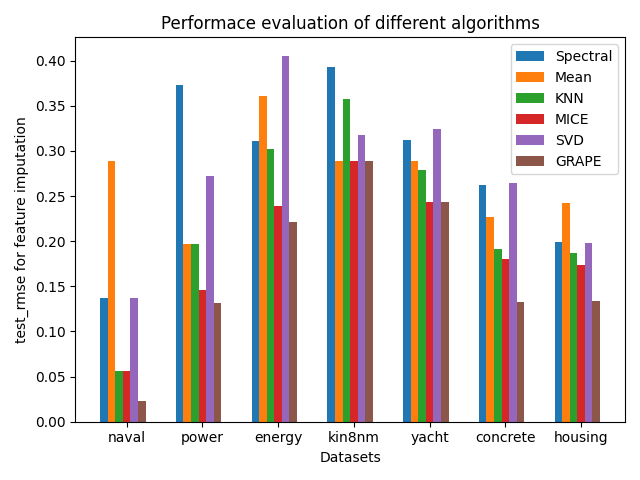
\includegraphics[width=1\textwidth]{figures/barplot_all.png}
 	\caption{Comparision of different methods for imputation}
 	\label{cdft}
 \end{figure}
\testbf{Label prediction:} The labels are randomly split into 70/30\% training and test sets. Figure 5 shows actual data from concrete dataset and values predicted by GRAPE on the dataset.
Further analysis on label prediction is yet to be done.
  \end{block}

\end{column}
\separatorcolumn
\begin{column}{\colwidth}
\vspace{-1cm}
    \begin{figure}
 	    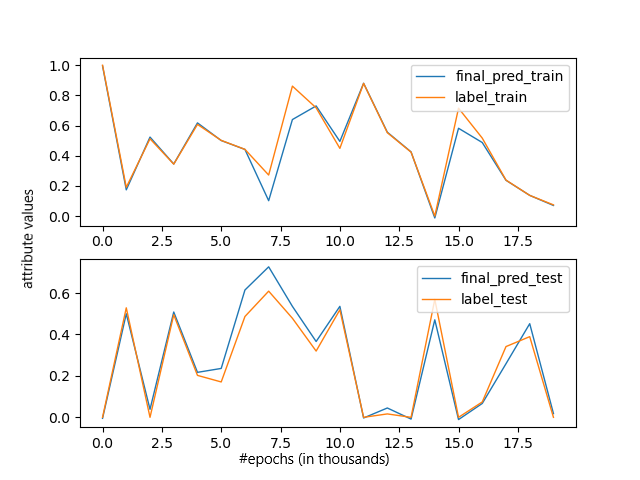
\includegraphics[width=1\textwidth]{figures/label_test.png}
 	    \caption{Label prediction for train and test sets}
 	    \label{cdft}
    \end{figure}
  \begin{block}{Results}
As shown in Figure 4, GRAPE has the lowest \textit{rmse} among all methods on all datasets.  For feature imputation, GRAPE gives 12\% lower average \textit{rmse} than the best bestline model (MICE).
 
  \end{block}

  \begin{block}{Conclusion}
In this project, GRAPE, a graph-based approach to handle missing data is introduced. It represents feature imputation as an edge-level prediction task and the label prediction as a node-level prediction task in a bipartite graph. Using these representations, it trains GNN to solve the tasks.

From the experiments on seven UCI datasets, the performance (\textit{feature imputation}) of GRAPE is seen to be significantly better (lower \textit{rmse}) than existing state-of-the-art methods.
  
  \end{block}
\begin{block}{Future Works}

\begin{itemize}
    \item Analysis of label prediction by GRAPE
    \item Imputation of missing values in timeseries data
\end{itemize}

\end{block}
\vspace{-.5cm}
\begin{block}{Acknowledgments}
\begin{scriptsize}
We are thankful to UCI Machine Learning Repository for the datasets and to Ohio Supercomputer Center (OSC) for GPU computing services.
\end{scriptsize}
\end{block}
\vspace{-.5cm}
\begin{block}{References}
\begin{scriptsize}
\textit{Handling Missing Data with Graph Representation Learning.} Jiaxuan You, Xiaobai Ma, et. al. Neural Information Processing Systems (NeurIPS), 2020.
\end{scriptsize}
\end{block}


\end{column} % 2 and 3
\end{columns}
\end{column} %\twocolwidth

\separatorcolumn
\end{columns}
\end{frame}
\end{document}
